\documentclass[letterpaper,10pt,conference]{ieeeconf}
\IEEEoverridecommandlockouts
\overrideIEEEmargins

\usepackage[utf8]{inputenc}
\usepackage[T1]{fontenc}
\usepackage{import}

\usepackage{xcolor}
\usepackage{xspace}

%these commands are used to make ieeeconf play nice with amsthm
\makeatletter
\let\IEEEproof\proof
\let\IEEEendproof\endproof
\let\proof\@undefined
\let\endproof\@undefined
\makeatother

\usepackage{amsmath,amssymb,amsthm}
\usepackage{graphicx,url}
\usepackage{microtype}
\usepackage{cleveref}
\usepackage{csquotes}
\usepackage{siunitx}
\usepackage{bm}
\usepackage{subcaption}

\usepackage{algpseudocode}
\usepackage{algorithm}
\usepackage{float}



\usepackage{placeins}

\usepackage[style=ieee,citestyle=numeric-comp]{biblatex}
\addbibresource{../../../../bibliography/bibliography.bib}

\renewcommand{\vec}[1]{\bm{#1}}
\newcommand{\R}{{\mathbb{R}}}
\DeclareMathOperator{\diag}{diag}
\DeclareMathOperator{\atantwo}{atan2}


\urldef{\you}\url{astoecke@uwaterloo.ca}

\title{Evaluation of Modern Reinforcement Learning Algorithms\\in the Context of Speech Resynthesis}
\date{August 1st, 2018}
\author{Andreas Stöckel\thanks{}
  \thanks{The author is with the Cheriton School of Computer Science and the Centre for Theoretical Neuroscience, University of Waterloo, Waterloo ON, N2L 3G1 Canada (\you)}}


\begin{document}

\maketitle

\begin{abstract}
Speech resynthesis is the process of approximately reproducing a speech signal with a speech synthesiser. In the particular case of an articulatory synthesiser---a physical model of the human vocal tract---speech resynthesis can be modelled as a reinforcement learning problem with a continuous state- and action-space. However, as of now, research in this area did not evaluate the performance of modern reinforcement learning algorithms. In this project report I provide an overview of prior work in the area of reinforcement learning based articulatory speech resynthesis, describe a novel OpenAI Gym learning environment implementing this task, and compare the performance of the ACKTR, DDPG, PPO and TRPO algorithms. Unfortunately, the results indicate that these algorithms cannot solve this task satisfactorily in the given environment and tend to converge towards sub-optimal control policies.
\end{abstract}

\section{Introduction}
\label{sec:introduction}

Most speech synthesis systems implement text-to-speech, that is, they translate a sequence of characters into an intelligible speech waveform. Here, I focus on a different aspect of speech synthesis, that in the above nomenclature might be called \enquote{speech-to-speech}. Given a speech waveform as an input, the task is to control a speech synthesiser in such a way that the output resembles the input. In other words, we would like to \emph{resynthesise} the original speech signal.

Typical text-to-speech systems operate in two phases. First, they derive a phonetic representation of the input text. Second, this phonetic sequence is converted to a sequence of control vectors for the actual speech synthesiser, which then produces the final audio waveform. Since speech-to-speech systems are already provided with an input that contains all phonetic information, these systems do not depend on the first phase, but directly control the synthesiser.

Common synthesiser architectures include concatenative synthesis, formant synthesis, articulatory synthesis, or, more recently, end-to-end trained deep neural networks such as WaveNet \cite{vandenoord2016wavenet}. As the name suggests, \emph{concatenative synthesis} is based on the concatenation of pre-recorded phoneme clusters. \emph{Formant synthesis} is based on additive superposition of parametrically filtered prototypical signals, for example a pulse train for vowels and white noise for fricatives. \emph{Articulatory synthesis} expands upon this method by implementing a more faithful model of the human vocal tract, and at least in theory, provides the best speech quality out of these three methods. However, the vocal-tract model is often simplified to reduce computational complexity, resulting in a \enquote{robotic sound}, while at the same time, correctly controlling individual articulatory synthesiser parameters---which can be thought of muscle tension in, or, more broadly speaking, the configuration of the vocal tract---has proven to be difficult. Correspondingly, commercial text-to-speech systems are often based on concatenative synthesis, or, nowadays, the aforementioned deep neural networks. Still, for the purpose of this project, I focus on controlling an articulatory synthesiser, which, in the context of speech-resynthesis, can be naturally phrased as a partially observable reinforcement learning problem.

It is not obvious why speech-resynthesis is an interesting problem. After all, if we already have access to a perfectly fine speech signal, why should we pass it through a synthesiser and obtain a signal of likely inferior quality? Foremost, speech resynthesis can be seen as a form of data compression. In some environments, such as mines/caves or under water, it is not possible to establish high-bandwidth radio links. Still, it may be advantageous to have access to intelligible voice transmissions \cite{barkand2006throughtheearth}. By acting as a \enquote{data-bottleneck}, or auto-encoder, speech resynthesis---in contrast to general-purpose audio compression schemes---has the potential to encode voice at data rates of a few hundred bits per second. Furthermore, the acoustic-to-articulatory inversion performed by the system can be seen as speech-features which can for example be used in speech recognition systems \cite{kirchhoff2002combining,prom-on2013training}.

Another application of speech-resynthesis is speaker transfer and anonymisation. Instead of faithfully reproducing the original signal, we can tune the parameters of the speech synthesiser to more closely resemble another person (\emph{transfer}) or sound more \enquote{robotic} (\emph{anonymisation}), for example to hide a person's identity in a radio or television interview.

Lastly, and especially in combination with an articulatory synthesiser and reinforcement learning, speech-resynthesis can be seen as a model of language acquisition during child-development. Just as a child must learn to control its vocal tract to reproduce perceived utterances, we are attempting to implement an algorithm which learns an acoustic-articulatory mapping, to turn utterances into a series of motor commands.

Previous work regarding speech-to-speech synthesis and acoustic to articulatory mapping is rather unsatisfactory in that it has only been applied to individual phonemes or short words; the question this work tries to answer is whether modern RL algorithms help to improve upon this status quo. I review both previous work and provide a quick description of the tested RL algorithms in \cref{sec:background}, followed by an outline of the particular methods used in this project in \cref{sec:method}. \Cref{sec:experiments} discusses a series of experiments, followed by a closing discussion and conclusion in \cref{sec:conclusion}.

\section{Background}
\label{sec:background}

This section reviews existing work in the field of speech resynthesis, provides an overview of the MFCC feature descriptors commonly used in speech processing, as well as a description of the reinforcement learning algorithms used in the experiments.

\subsection{Speech Resynthesis}

Speech resynthesis is a complex, high-dimensional control task in a continuous action space. It is closely related to the problem of acoustic-to-articulatory inversion---finding the inverse function that maps from a speech signal onto articulatory space. While it is possible to fit a function with labelled datasets mapping from acoustic space directly onto the ground-truth articulatory poses \cite{uria2011deep}, for example using Electromagnetic Articulography (EMA) recordings \cite{birkholz2007control}, producing these data is relatively expensive. Still, work in this area often relies on an initial supervised training with subsequent unsupervised refinement. 

Such an approach is for example pursued in \cite{philippsen2014learning}, which first independently trains two RNNs $f$ and $g$ to perform the forward and inverse acoustic to articulatory mapping, respectively. After this initial training, the agent is presented with an acoustic signal and uses $g$ to compute the estimated articulatory poses, which are transformed to acoustic space using the articulatory synthesiser VocalTractLab \cite{birkholz2017vocaltractlab}. The perceived output signal is then used to update both $f$ and $g$ chained into single, auto-encoder like neural network. This approach significantly improves the inverse model, however, the authors only report results for phoneme pairs and not for words or sentences.

A mostly unsupervised method is presented in \cite{prom-on2013training}. Here, segmented (along phoneme boundaries) audio samples are converted to sequences of MFCC features (see below). For each segment, the parameters of the articulatory synthesiser are initialised randomly and optimised by stochastic gradient descent combined on the loss function defined by the mean square error of the input MFCC sequence and the output MFCC sequence, as proposed in \cite{mermelstein1976distance}. This method is capable of learning to imitate entire words.

A reinforcement learning based approach applied to the imitation of vowels is presented in \cite{murakami2015seeing}. Inspired by infant speech acquisition, the authors first train an unsupervised auditory memory model that stores prototypical utterances. The agent then selects one of these utterances as a target and starts to activate its control output based on a randomly initialised policy function---the agent \enquote{babbles}. A scalar value indicating the between the output utterance and the prototype as produced by the auditory memory is fed back to the agent as a reward signal. The agent uses the \emph{Covariance Matrix Adaptation Evolution Strategy} (CMA-ES) method to adapt its policy function. Given some \enquote{visual} input (i.e.,~lip shape and jaw location), the method successfully learns to imitate the vowels $/u/$, $/a/$, and $/i/$.

The above methods train phonemes individually. This might be a clear warning that learning the acoustic-to-articulatory inversion is a hard problem. Nevertheless, in the following I would like to explore how well modern reinforcement learning techniques---solving seemingly complex tasks such as playing Atari games or learning to walk---cope with learning articulatory inverse mapping based on complex speech signals.

\begin{figure*}[t]
	\centering
	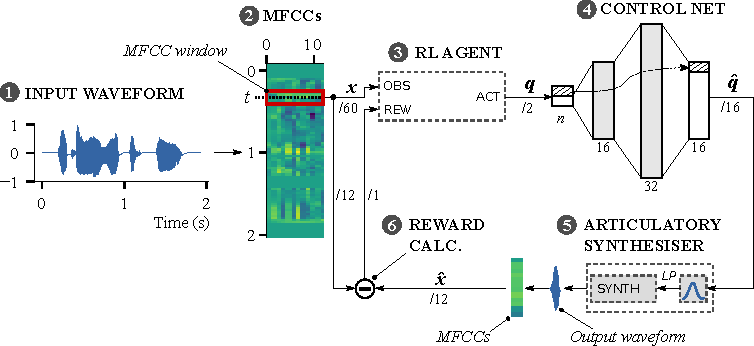
\includegraphics{media/overview.pdf}
	\caption{Architecture of the speech-to-speech system. Everything outside the \enquote{RL agent} box constitutes the environment. The notation \enquote{$/d$} describes the dimensionality of the individual vectors. See text for a more detailed description.}
	\label{fig:architecture}
\end{figure*}

\subsection{Reinforcement Learning}

I evaluate four modern continuous action reinforcement learning algorithms provided as part of the \enquote{OpenAI Gym Baselines} package, originally controlling a continuous action space MuJoCo environment. The algorithms are used as-is in this project, without any modification to the original source code. In the following, I summarise the key ideas behind each algorithm.

\emph{Deep Deterministic Policy Gradients:} The DDPG algorithm for continuous control has originally been published in 2015 \cite{lillicrap2015continuous}, and is inspired by the success of \emph{Deep $Q$ Networks} (DQNs). While DQNs can handle high dimensional, continuous observation spaces, their action space is intrinsically discrete. DDPG extends the Deterministic Policy Gradient algorithm by replacing both the parametrised actor function $\pi(s)$ and the critic $Q(s, a)$ with \enquote{deep} neural networks. Introduction of these non-linear function appropriators no longer guarantees convergence to the optimal policy. DDPG therefore employs a replay buffer, as well as a soft update of the target network parameters $\pi'$, $Q'$. Exploration is modelled by adding Gaussian noise to the actions selected by $\pi(s)$. DDPG has been successfully applied to complex control problems such as \enquote{learning to walk} and steering a video game car by interpreting from raw pixel data.

\emph{Trust Region Policy Optimization:} Similar to policy gradient methods, TRPO \cite{schulman2015trust} maintains a parametrised policy function $\pi(s)$ in the form of a neural network. However, TRPO does not optimize the policy parameters by following a gradient, but instead maximises a constrained surrogate function based on trajectories of state, action, and reward pairs using the conjugate gradient method. The surrogate function is guaranteed to optimize the policy in a local environment, the trust region. Since the optimization process takes multiple samples into account, TRPO is more sample efficient than na\"ive policy gradient methods. TRPO has originally been applied to continuous locomotion problems.

\emph{Proximal Policy Optimization:} PPO is a relatively new algorithm originally presented in 2017 \cite{schulman2017proximal}. PPO seeks to combine the benefits of TRPO, namely sample efficiency, with a considerably simpler implementation not relying on higher order derivatives. PPO alternates sampling and gradient-based policy optimization of a surrogate function from a replay buffer. While PPO is easier to implement, it outperforms all other RL algorithms for continuous control on the locomotion tasks.

\emph{Actor Critic using Kronecker-Factored Trust Region:} The 2017 algorithm ACKTR \cite{wu2017scalable} further improves the computational cost and sample efficiency of TRPO by approximating the curvature of the surrogate function using \enquote{Kronecker-factored approximated curvature}. ACKTR furthermore adopts the actor-critic mechanism and can be applied to large neural networks due to a relatively cheap update step. ACKTR clearly outperforms other algorithms in discrete action spaces, such as Atari games, and exhibits an excellent performance in continuous control tasks such as the aforementioned locomotion environments.

\subsection{MFCC Speech Feature Extraction}

Speech feature extraction usually relies on a model of human psychoacoustics---intuitively, machine-based speech processing should be based on information similar to what is available to the human nervous system. In essence, the human auditory system processes sound waves in the short-time frequency domain. While more sophisticated models of the auditory system along with corresponding feature descriptors exist \cite{murakami2015seeing}, I focus on the \emph{Mel Frequency Cepstral Coefficients} \cite{mermelstein1976distance}, commonly used in speech recognition systems.

In mammals, the transformation from a time-varying amplitude signal to frequencies is purely mechanical and relies on the physical properties of the \emph{cochlea}, a conical, fluid-filled tube in the inner ear. In contrast to short-time frequency transforms based on the Fourier transformation, the space spanned by the cochlea is not linear on the frequency axis. The ear is more sensitive to small absolute changes in pitch of lower frequencies compared to higher frequencies.

This non-linearity is captured by the \emph{Mel} scale and the corresponding Mel spectrogram, which is computed by keeping a sliding window of audio data. In regular intervals the data transformed to frequency space using the discrete Fourier transformation. The power spectrum (absolute values) of the resulting coefficients is then collapsed into fewer bands according to the Mel scale. This results in a---usually---forty-dimensional spectrogram slice every few milliseconds. In a last step, the coefficients are transformed to a logarithmic $\mathrm{dB}$ scale. See \cref{fig:control_network_spectrogram} for an example.

Natural sound waves, and vowels in speech in particular, are rich in harmonic content. That is, if a frequency $f_0$ is present in the spectrogram, then it is likely to find the harmonic frequencies $f_n = n \cdot f_0$, for $n \in \mathbb{N}^+$. In other words, the individual spectrogram slices are highly correlated, unnecessarily increasing the dimensionality of the input signal. Two common ways to linearly decorrelate the spectrogram are to project the spectrogram slices onto the first principal components of a large sample of spectrogram slices, or to decorrelate the signal by computing the discrete cosine transform (DCT) of the spectrogram slice%
\footnote{The DCT is regularly used to linearly decorrelate natural signals, since their principal components closely resemble the DCT basis.} and discarding higher-order coefficients, resulting in the MFCC vector. The MFCCs implicitly capture interesting features of the speech signal, such as the fundamental frequency $f_0$, as well as the formant structure (the intensity peaks of the harmonics), which is essential for vowel discrimination. See \cref{fig:control_network_mfccs} for an example.

\section{Method}
\label{sec:method}

The system architecture is partly inspired by \cite{prom-on2013training,murakami2015seeing} and depicted in \cref{fig:architecture}. The task is a partially observable reinforcment learning problem---the agent does not have access to the hidden state of the environment. In other words, the agent does not have access to the hidden articulatory configuration of the speaker, but only her acoustic signal. During each training episode, the \emph{environment} selects a speech waveform, which is decomposed into a time-series of MFCC feature vectors. A sliding window of MFCCs is presented as observation to the reinforcement learning agent; providing a window of MFCCs allows the agent to compensate for latencies in the signal processing pipeline by incorporating past and future input data. To reduce the control dimensionality, the agent generates a continuous, low-dimensional action $\vec q \in \mathbb{R}^n$ which is then translated by the \emph{control network} to the actual 16-dimensional input $\vec{\hat q}$ of the articulatory synthesiser. The environment captures the output of the synthesizer and computes the corresponding MFCC features, which are then compared to the input according to their root mean square error (RMSE), resulting in the reward signal $r$. The following subsections describe these individual components in more detail.

\subsection{Environment and Speech Samples}

The environment is implemented as an OpenAI gym environment and relies on two datasets for speech samples. The first dataset encompasses artificial speech data generated by the TRM itself using the control trajectories generated by the text-to-speech component of \emph{gnuspeech}. The articulatory synthesiser included in the environment should theoretically be capable of perfectly reproducing these samples (except for errors introduced by the control network, see below). The second dataset encompasses five audio books with both male/female speakers sourced from the LibriVox\footnote{Public-domain audio books; see \url{https://librivox.org/}.} project.

In a preprocessing step, the PCM speech data is automatically segmented into $0.5$-$10\,\mathrm{s}$ long chunks, where each chunk corresponds to one training episode. At the end of every episode, the synthesiser is reset to its original state. Segment boundaries are located at longer stretches of silence, ensuring that the dataset only contains complete utterances. The corresponding MFCCs  (based on a $512$ sample window at $16\,\mathrm{kHz}$ sample rate, corresponding to $32\,\mathrm{ms}$; one MFCC vector every $128$ samples, corresponding to $8\,\mathrm{ms}$; 12 dimensions per MFCC) are precomputed and stored alongside the PCM data. There are $4946$ chunks at $6$ hours of audio in the first dataset, and $62\,840$ chunks at $45$ hours in the second dataset.

\subsection{Articulatory Synthesiser}

The articulatory synthesiser used in this project is derived%
\footnote{I adapted the \emph{gnuspeech} source code to include a C API for the TRM with a corresponding Python binding. To reduce latencies I exchanged the resampler translating from the TRM resonance freqency to the audio sample rate with \emph{libspeexdsp}. Code is available at \url{https://github.com/astoeckel/gnuspeech_trm}.}
from \emph{gnuspeech} \cite{hill1995realtime,hill2015gnuspeech} and implements the \enquote{Tube Resonance Model} (TRM) originally developed in the early 1990s. In contrast to more modern articulatory synthesisers (e.g. BOSS \cite{prom-on2013training}, or VocalTractLab \cite{birkholz2017vocaltractlab}), \emph{gnuspeech} has the advantage of being relatively simple and extremely fast on modern hardware, which facilitates a high-throughput exploration of the articulatory space. As discussed in \cite{manzara2005tube}, the TRM is a model of the throat (oropharynx) and nasal cavities. These cavities are divided into a number of segments acting as waveguides. The synthesiser simulates longitudinal sound waves emitted by the vocal cords (glottis), which travel along and are reflected within these segments. The radii of the eight oropharynx segments are available as parameters and model the position of the tongue as well as mouth shape. Furthermore, noise sources corresponding to aspiration sound and fricatives are available; the \enquote{fricative} noise can be band-pass filtered and injected at any location of the oropharynx.

In total, the synthesiser is driven by 16 control parameters (see \cref{fig:control_parameters} for a list). Note that the control input is low-pass filtered with a $20\,\mathrm{ms}$ moving-average filter, adding latency to the control problem.

\subsection{Control Network}

\begin{figure}
	\centering
	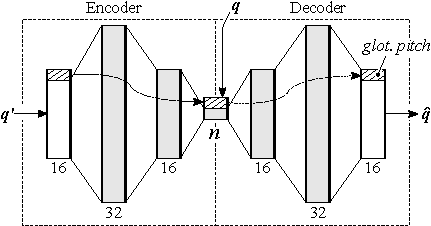
\includegraphics{media/control_network.pdf}
	\caption{Sketch of the control network. Shaded boxes correspond to non-linear neuron layers ($\tanh$-nonlinearity), numbers to the dimensionality/number of neurons in that layer. Connections are all-to-all. The first component of the control vector $\vec x$ (the glottal pitch; hatched boxes) is passed through, since it is independent of the other controls. After being trained, only the right half of the network is used, input is passed in through $\vec{q}$.}
	\label{fig:control_network}
\end{figure}

\begin{figure*}[p]
	\begin{subfigure}[t]{\textwidth}
		\centering
		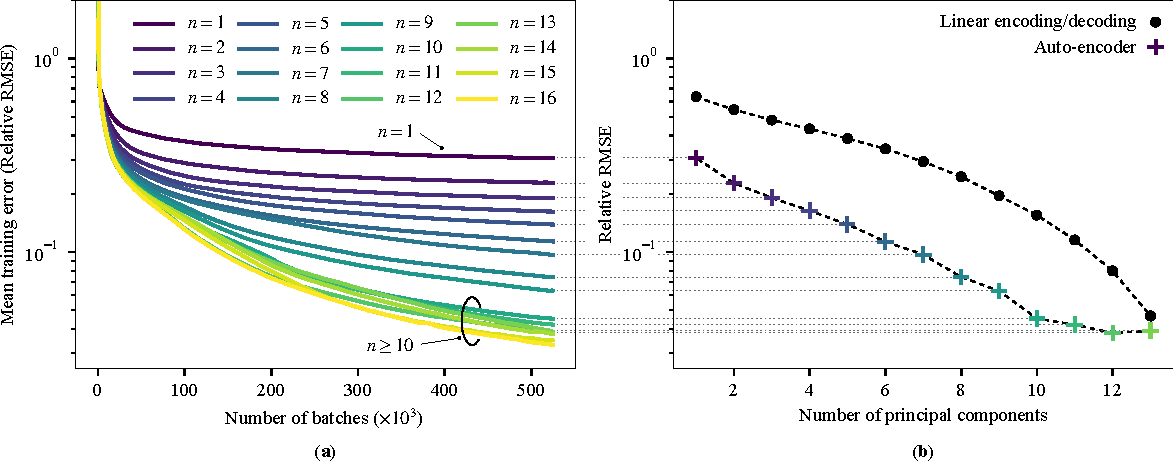
\includegraphics[scale=0.825]{media/control_network_training_pca.pdf}
		\phantomcaption
		\label{fig:control_network_training}
	\end{subfigure}
	\begin{subfigure}[t]{0\textwidth}
		~
		\phantomcaption
		\label{fig:control_network_pca}
	\end{subfigure}
	\caption{\textbf{(a)} Average (16 trials) relative RMS batch training error for the auto-encoder control network for various bottleneck sizes $n$. One batch corresponds to $512$ randomly sampled control vectors out of $5\,438\,562$ (RMS is $\approx 0.64$). \textbf{(b)} Comparison between the auto-encoder network and PCA. Note that the error is zero for $n \geq 14$ principal components.}
\end{figure*}

\begin{figure*}[p]
	\begin{subfigure}[t]{\textwidth}
		\centering
		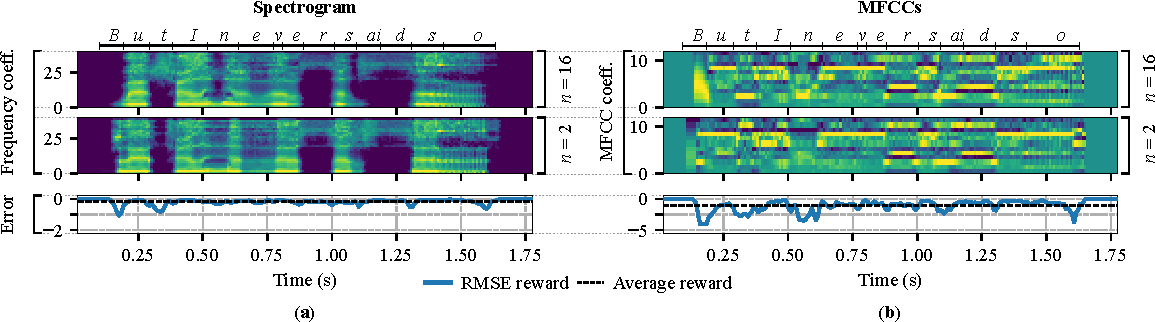
\includegraphics[scale=0.825]{media/control_network_spectrogram.pdf}
		\phantomcaption
		\label{fig:control_network_spectrogram}
	\end{subfigure}
	\begin{subfigure}[t]{0\textwidth}
		~
		\phantomcaption
		\label{fig:control_network_mfccs}
	\end{subfigure}
	\caption{Utterance produced with $n = 16$ parameters, compared to the auto-encoder model ($n = 2$, pitch and scalar control value). \textbf{(a)} Mel spectrogram, \textbf{(b)} MFCC feature vectors. Bottom: reward based on the similarity between the spectrogram/MFCCs.}
	\label{fig:control_network_one_dim}
\end{figure*}

\begin{figure*}[p]
	\centering
	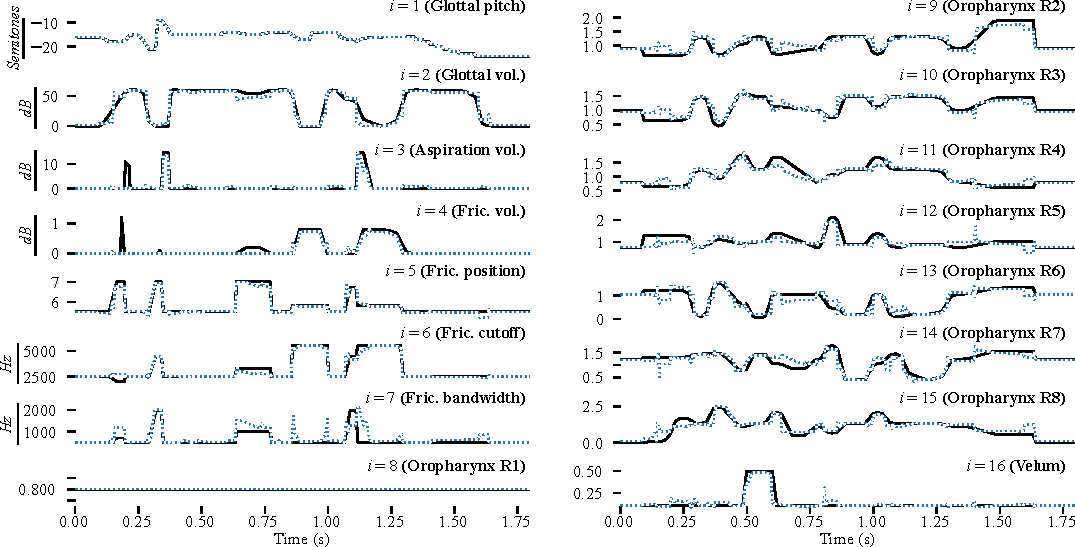
\includegraphics[scale=0.825]{media/trm_params.pdf}
	\caption{Original control trajectories (black) compared to the one-dimensional (excl.~pitch) approximation (dotted, blue). Diagram corresponds to the same utterance as the one shown in \cref{fig:control_network_one_dim}.}
	\label{fig:control_parameters}
\end{figure*}

As mentioned in the introduction, one of the major issues of articulatory synthesis is the relatively high-dimensional control vector ($16$ dimensional in the case of the TRM; all parameters normalised to $[-1, 1]$). Not only is infeasible to exhaustively explore a 16-dimensional hypercube, but it is also not very efficient, since the vast majority of parameter configurations will not result in any intelligible output. For example, setting any of the tube radii $r_1, \ldots, r_8$ to a value close to zero will prevent sound from propagating. Furthermore, some parameter combinations are impossible due to embodiment constraints \cite{prom-on2013training}, for example, the tongue can only block some portions of the oral cavity, but not all. A reinforcement learning agent would implicitly have to learn a manifold inside the higher-dimensional space which corresponds to the subspace of sensible control parameters. Preliminary experiments indicated that none of the RL algorithms made significant progress on this problem within a few hours of training.

One solution to this problem is to manually reduce the parameter space dimensionality. To uncover the underlying manifold, we can analyse a set of control vectors sampled from the text-to-speech module that normally drives the TRM. Here, I employ a non-linear auto-encoder network with variable bottleneck dimensionality compared to a linear decorrelation based on principal component analysis as a baseline. Perhaps unsurprisingly, an initial observation is that the glottal pitch parameter is mostly independent of the other parameters, i.e., it is possible to speak the same utterance at various pitches. I therefore separate the glottal pitch from the other parameters before training. The architecture of the auto-encoder control network is sketched in \Cref{fig:control_network}, the network is trained using the Adam back-propagation algorithm with batches of 512 randomly selected samples from the same control trajectories used to produce the artificial training dataset. The training progress is shown in \cref{fig:control_network_training}; a comparison to a linear decorrelation in \cref{fig:control_network_pca}. As clearly visible, for more than $n \geq 10$ parameters the achieved training error for auto-encoder is negligibly small, suggesting that the intrinsic dimensionality of the samples is about ten dimensional. Still, for $n = 1$ control dimension (excluding the pitch) the auto-encoder achieves an error that corresponds to using about seven principal components with linear decorrelation. Essentially, for $n = 1$ the auto-encoder smoothly arranges vowels, consonants, and pauses onto the interval $[-1,1]$. \Cref{fig:control_network_one_dim} demonstrates that a two-dimensional control scheme (pitch and the one-dimensional control) still allows us to reproduce the output produced with the full control vector (average reward is about $-0.9$ versus $-2.9$ for random babbling). I will therefore employ this two-dimensional control scheme in subsequent experiments.

\subsection{Reward Computation}

The reward $r$ passed to the RL agent is computed similarly to the method presented in \cite{prom-on2013training} and simply corresponds to the negative root mean square error (RMSE) between the MFCC vector $\vec{\hat x}$ extracted from the articulatory synthesiser output and the MFCC vector $\vec{x}$ at the centre of the MFCC window presented to the RL agent
\begin{align}
	r &= - \| \vec x - \vec{\hat x} \|_2 \,.
	\label{eqn:reward}
\end{align}
Note that the MFCC vectors are not speaker independent, since they implicitly capture the fundamental frequency (pitch) $f_0$, which, for example, depends strongly on sex and age of the speaker. Correspondingly, in order to maximize the reward, the agent must learn to select the correct pitch.


\begin{figure*}[p]
	\centering
	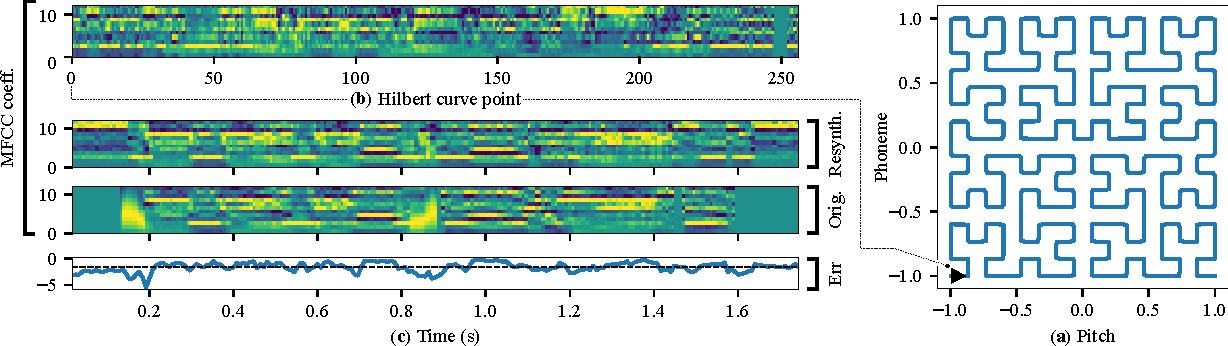
\includegraphics[scale=0.825]{media/hilbert.pdf}
	\caption{Pilot experiment overview. \textbf{(a)} Control trajectory along a space-filling Hilbert curve used to sample the prototypical MFCCs depicted in \textbf{(b)}. \textbf{(c)} utterance (bottom) resynthesised (top) by choosing the control point on the Hilbert curve associated with the prototypical MFCC most closely matching the input MFCC.}
	\label{fig:hilbert}
\end{figure*}

\begin{figure*}[p]
	\centering
	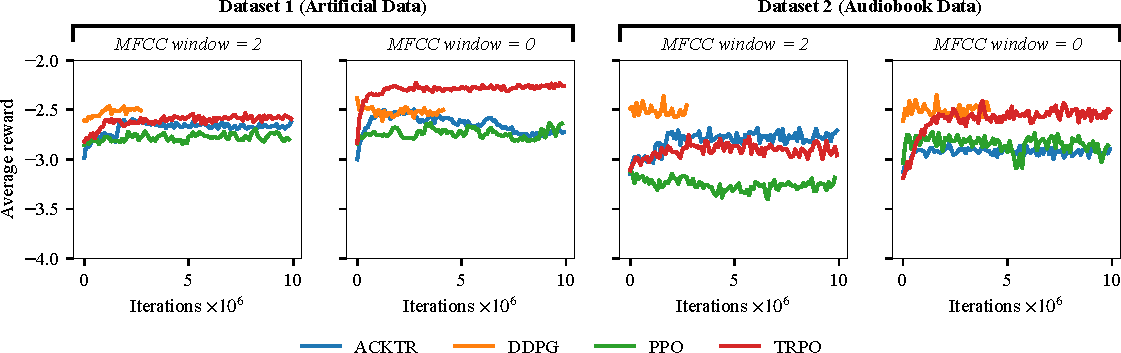
\includegraphics[scale=0.825]{media/results.pdf}
	\caption{Average training reward per iteration for the four reinforcement learning algorithms over $10$ million training iterations (except for DDPG). Averages are over $100\,000$ iterations.}
	\label{fig:results}
\end{figure*}

\begin{figure*}[p]
	\centering
	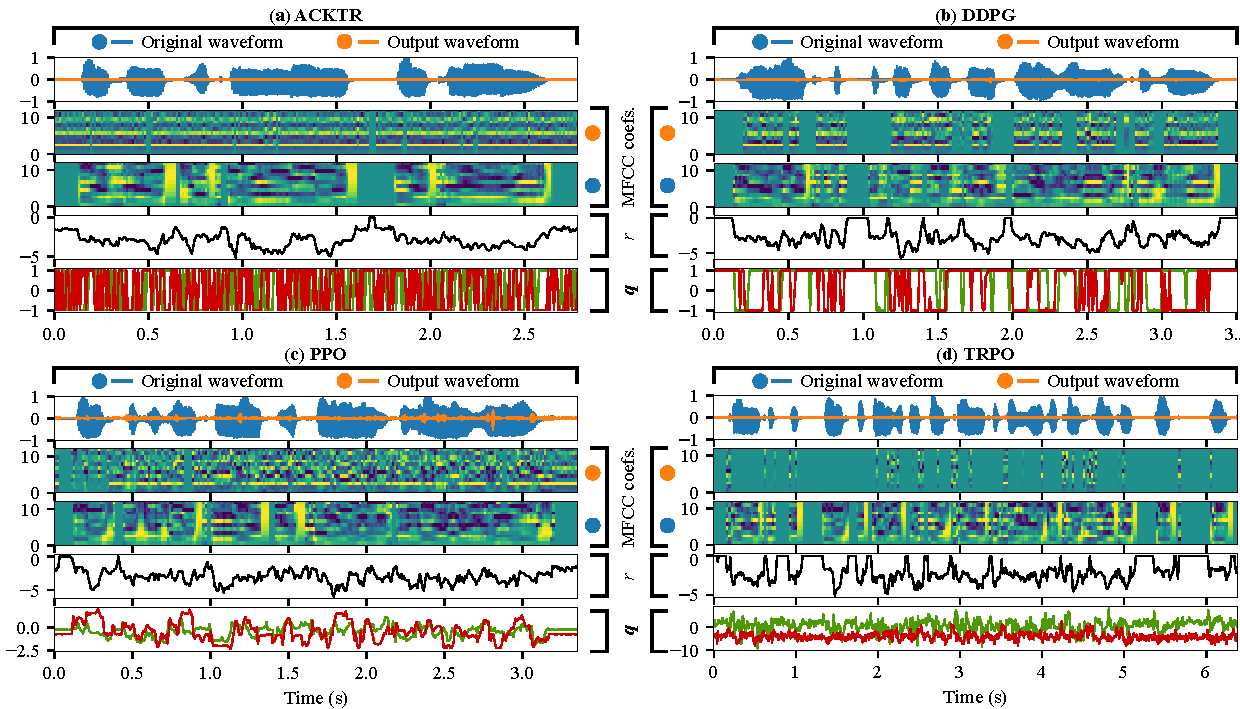
\includegraphics[scale=0.825]{media/results_examples.pdf}
	\caption{Collection of final training episodes showing the waveforms, MFCCs, reward $r$, and control trajectories $\vec q$ over time.}
	\label{fig:results_examples}
\end{figure*}

\section{Experiments and Results}
\label{sec:experiments}

The first experiment, depicted in \cref{fig:hilbert}, verifies that, at least in the case of the artificial dataset, it is in theory possible to perform intelligible speech re-synthesis. To this end, I traverse the two-dimensional control space along a Hilbert curve on a $16 \times 16$ grid. This control trajectory is synthesised and the corresponding MFCCs are computed; as a result, each point on the Hilbert curve is associated with an MFCC vector. In a second step I load a subset the MFCCs corresponding to the artificial dataset. I resynthesise these samples by selecting the sample point on the Hilbert curve with the closest MFCC according to \cref{eqn:reward}. This very simple scheme results in a mostly intelligible resynthesis at an average reward of $-2.47$ over $75\,460$ iterations. However, for individual phonemes this error reaches rewards close to the optimal value of zero. Considering the relative coarse exploration scheme employed in this experiment, it should be possible for a reinforcement learning algorithm to find good control outputs for at least some phonemes.

\Cref{fig:results} depicts the average reward per iteration over ten million training iterations for both datasets with varying MFCC window size $w$ set to two and zero. This last variation is meant to explore whether access to future and past MFCCs is useful. Note that training was aborted for DDPG because of comparably slow training. Except for TRPO for $w=0$, there is no significant increase in the agent performance. For $w = 0$ and the artificial dataset, TRPO starts at the \enquote{random babbling} baseline performance of $-3$ and achieves an average reward of $-2.3$, which is considerably better than the performance of the simple heuristic in the above pilot experiment. Choosing $w = 2$ seems to degrade the performance slightly, either suggesting that the input dimensionality is too large or that past and future MFCCs do not contain useful information.

However, recordings of the training sessions---excerpts shown in \cref{fig:results_examples}---reveal that in none of the experiment any agent is capable of reproducing an intelligible speech signal. Instead, the agents seem to have converged to a state where they produce a near-silent \enquote{sizzling}, with TRPO producing complete silence most of the time. Since silence perfectly matches silence in the input recording, this behaviour is highly rewarded whenever the two coincide. Moreover, and although the RL implementations originally drove the same MuJoCo environment and should thus be set to the same output range, ACKTR and DDPG generate action signals that lie outside $[-1, 1]$, and are correspondingly clipped to the boundaries. The relatively large average reward for DDPG seems to be caused the relatively steady action signal, while generating silence at appropriate times.

Since none of the agent implementations shows the desired behaviour, it is hard to evaluate the strengths and weaknesses of the individual algorithms. Instead, and as discussed below, the results seem to suggest that the current reward function is suboptimal, making it too hard to find the optimal output while \enquote{encouraging} undesired policies.

\section{Discussion and Conclusion}
\label{sec:conclusion}

The previous sections outlined speech resynthesis---learning to speak by imitation---as a reinforcement learning task and described an implementation of a corresponding system architecture, as well as a series of experiments employing modern RL algorithms to solve this task.

Alas, the results are mildly disheartening. It is quite surprising that none of the algorithms is even capable of resynthesising the artificial speech dataset with an error small enough to count as \enquote{intelligible}. This is even more puzzling taking into account the problem has been considerably simplified by implicitly encoding the phonemes present in the artificial dataset in the control network, from where they, as demonstrated in the pilot experiment, can be reconstructed by merely providing the \enquote{correct} scalar value. Thus, this two-dimensional control problem (finding the correct phoneme and the correct pitch) appears to be easier than learning to play an Atari game, or controlling a many-DOF body.

From analysing traces, there are two major problems. First, the reward function is compatible with some unexpected solutions, such as the \enquote{silent whisper} found by TRPO, while penalising intelligible solutions, such as the ones found in the pilot experiment, too strongly. Second, the algorithms seems to be \enquote{stuck} in local minima: while it should be possible to improve beyond  in certain contexts, some actions provide a relatively large reward beyond which the algorithms fail to improve. Both problems are to some degree this may be caused by the MFCC-based reward function. MFCC similarity is a good measure for two signals being close in frequency space, but, although they have been invented for this purpose \cite{mermelstein1976distance}, do not necessarily correspond to two signals being perceived as the same phoneme. Correspondingly, a future step forward may be to compute the reward with a \enquote{reward network}, that has been trained to score the similarity of phonemes produced by various speakers/differently configured synthesisers.

The mere choice of MFCCs as feature vectors may be criticised. Experiments with convolutional neural networks demonstrated repeatedly that implicit learning of features often achieves better performance than any hand-crafted feature detector. However, at least for this project, this was not an option due to limited computational resources.

In a similar vain, it is questionable whether the use of an articulatory synthesiser is in vogue, given that the entire setup could be replaced with a deep neural network and trained in a fully supervised way. Experiments with WaveNet and the low-bitrate speech codec \emph{Codec2} have recently demonstrated that such a setup is suitable for transmitting high-quality speech at extremely low bitrates \cite{bastiaankleijn2017wavenet}.

Apart from the reasons mentioned in the introduction, there are at least two reasons why the particular setup presented in this project is viable: computational efficiency and providing a benchmark for RL algorithms. Regarding efficiency, articulatory synthesisers such as the \emph{gnuspeech} TRM are highly optimised and can easily synthesise audio at a hundred times real time on modern computers; correspondingly, finding the correct control parameters to imitate speech would, in contrast to WaveNet, allow for a resource conserving decoder.

Furthermore, since this problem seems to be surprisingly hard (assuming that there are no bugs in my code), it may drive further development of RL algorithms, especially in the context of biologically inspired unsupervised learning; after all, from personal experience, both infants and parrots are well capable of solving this task. However, the initial results presented here should be taken with a grain of salt. More thorough experimentation and validation of the results as permitted by the scope of this project is required.

%\AtNextBibliography{\small}
\printbibliography

\end{document}